\chapter{Usikkerhet og signifikante sifre}
I motsetning til i matematikk der vi som regel kan anta at vi har eksakt kjennskap til størrelsene vi jobber med har vi i fysikk generelt bare kjennskap til størrelsen med en viss presisjon. Dette skyldes at fysiske størrelser har opphav i målinger og der kan vi aldri ha uendelig presisjon. Skal vi gjøre ting helt korrekt skal størrelsen oppgis sammen med dens estimerte usikkerhet.\footnote{Heller ikke usikkerheten er eksakt bestemt, men det er som regel mulig å estimere denne på en systematisk måte.
} For eksempel kan en lengde oppgis som $x=(1,03\pm0,02)~\mathrm{m}$. Dette betyr det beste estimatet vi har på lengden er $x = 1,03~\mathrm{m}$. Usikkerheten $\pm0,02~\mathrm{m}$ betyr at vi mener å vite at hvis denne lengden blir målt mange ganger vil flesteparten\footnote{Det vanligste er å bruke en definisjon av usikkerheten som gjør at 67\% at målingene skal havne innenfor intervallet definert av usikkerheten.} av målingene skal vise mellom $x=1,01~\mathrm{m}$ og $x=1,05~\mathrm{m}$. 

I regneoppgaver forholder vi oss vanligvis litt mer avslappet til usikkerheten i størrelsene, men vi glemmer den ikke helt. Hvis f.eks. en energi oppgis som $2,52~\mathrm{J}$ tolkes det som at usikkerheten er i det siste sifferet. Det kan altså tenkes at den riktige verdien er $2,51~\mathrm{J}$ eller $2,55~\mathrm{J}$, men sannsynligvis ikke at avviket er så stort at den riktige verdien er $2,60~\mathrm{J}$. En tommelfingerregel for å få en fornuftig presisjon i svaret av en beregning er å ikke ta med flere sifre i sluttsvaret enn det var i den inn-verdien med færrest sifre.

Noen få ord om hvordan man teller sifre: Hvis vi teller fra venstre er det første sifferet som er ulik 0 det første vi teller. Deretter teller alle sifre med i regnskapet. Eksempler:
\begin{itemize}
	\item 1,54 -- tre sifre
	\item 0,03 -- ett siffer
	\item$1,3\times10^6$ -- to sifre
\end{itemize}
Merk at hvis du får svaret $238~\mathrm{m}$ og kun skal ha med to sifre må svaret skrives som $2,4\times10^2~\mathrm{m}$ for å følge denne regelen siden å skrive det avrundete tallet $240~\mathrm{m}$ fremdeles er å skrive tre sifre.


\section{Estimering av usikkerhet}
Noen ganger er ikke tommelfingerregelen om antall signifikante sifre tilstrekkelig. For eksempel må usikkerhet behandles skikkelig hvis man skriver en vitenskaplig artikkel eller en teknisk rapport. Også i labøvinger er det vanlig å kreve at usikkerheten behandles på en ordentlig måte. 

\subsection{Ulike typer usikkerhet}
Det er vanlig å klassifisere måleusikkerhet i to kategorier: systematisk og statistisk. Den systematiske usikkerheten er direkte knyttet til måleinstrumentet eller metoden, og vil typisk gi feil i samme retning---altså for stor eller for liten verdi---hver gang dersom målingen gjentas. Et eksempel finner vi dersom vi skal måle bredden av en planke ved hjelp av en linjal. Den korrekte bredden finner vi dersom linjalen er plassert perfekt i $90\circ$ vinkel over planken. Dersom vinkelen ikke er helt riktig vil vi ende opp med å måle en bredde som er for stor, men det er ingen vinkel som gir for liten bredde. 

Statistisk usikkerhet beskriver det at enhver måling som forsøker å gå til grensen av nøyaktigheten som er mulig å oppnå med det aktuelle måle\-instrumentet alltid vil ha en viss variabilitet som typisk fordeler seg tilfeldig til begge sider av den sanne verdien. I de fleste tilfeller vil denne variasjonen beskrives godt som en gaussisk/standard-fordeling. 

Forholdet mellom systematisk og statistisk usikkerhet kan belyses ved å se på forskjellen mellom \emph{presisjon} og \emph{nøyaktighet} som er illustrert i figur \ref{fig:usikkerhet:presisjon}. Presisjon beskriver hvor godt gjentatte målinger stemmer overens med hverandre, slik at god presisjon henger sammen med en liten statistisk usikkerhet. Nøyaktighet beskriver hvor godt gjennomsnittet av mange målinger treffer den sanne verdien som vi prøver å finne ved hjelp av målingene. Nøyaktighet er derfor knyttet til systematisk usikkerhet. Som figuren viser kan vi ha f.eks. god nøyaktighet, men samtidig dårlig presisjon. Ideellt sett vil vi gjøre både nøyaktigheten og presisjonen så god som mulig, men det har liten verdi å gjøre den ene veldig god dersom den andre er dårlig.

\begin{figure}[htp]
	\begin{center}
		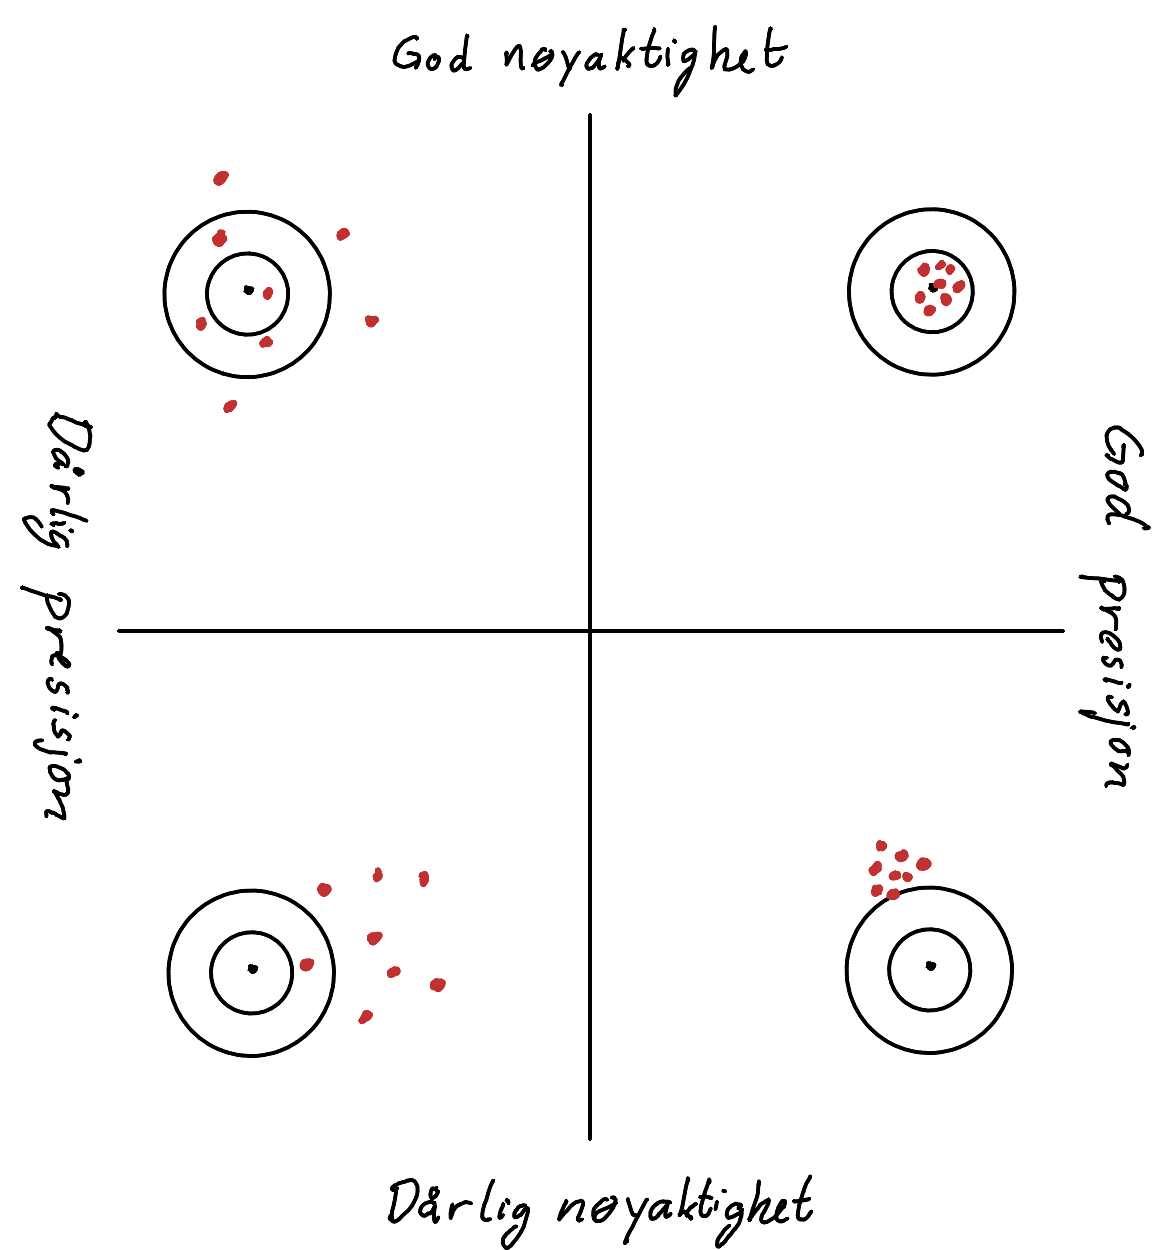
\includegraphics[width=.5\textwidth]{./presisjon}
	\end{center}
	\caption{Illustrasjon av forskjellen mellom begrepene nøyaktighet og presisjon. En god måling ønsker vi at skal være både nøyaktig og presis.}
	\label{fig:usikkerhet:presisjon}
\end{figure}


\subsection{Absolutt og relativ usikkerhet}
Avhengig av sammenhengen brukes to ulike måter å oppgi usikkerheten på: absolutt og relativ usikkerhet. Begge deler uttrykker det samme, det er bare ulike måter å presentere informasjonen på. Dersom vi har en lengde oppgitt som $x=(1,03\pm 0,02)\unit{m}$ da omtaler vi størrelsen $\sigma_x = 0,02\unit{m}$ den \emph{absolutte usikkerheten}. Denne har alltid samme enheter som størrelsen selv. Dersom vi er mer interessert i hvor stor usikkerheten er sammenlignet med den målte størrelsen selv gir vi heller den \emph{relative usikkerheten}: 
\begin{displaymath}
	\frac{\sigma_x}{x} = \frac{0,02\unit{m}}{1,03\unit{m}} = 0,019 = 1,9\%
\end{displaymath}
Siden den relative usikkerheten er et forholdstall har den ingen dimensjon, men oppgis enten som et desimaltall eller som prosent.

Det er ingen egentlige regler for når man skal bruke absolutt og når man skal bruke relativ usikkerhet, men det er mulig å gi noen tommelfingerregler. Hvis man har en enkelt størrelse oppgitt med usikkerhet, er det som regel den absolutte usikkerheten som er enklest å tolke. Dersom man derimot har behov for å sammenligne usikkerheten til målinger av størrelser med ulik benevning er det meningsløst å sammenligne absolutt usikkerhet (hva er størst usikkerhet, $\pm 3\unit{cm}$ eller $\pm 2\unit{^\circ C}$?). Derimot kan en slik sammenligning gjøres meningsfull ved å bruke relativ usikkerhet.

\begin{texample}
{\bf
Vi har $n=(0,022\pm0,001)\unit{mol}$ av en ideell gass i en beholder med volum $V = (5,00\pm0,01)\cdot 10^{-4}\unit{m^3}$. Vi måler trykket til å være $p=(1,035\pm0,011)\cdot 10^5\unit{Pa}$ og ønsker å regne ut temperaturen fra disse måledataene. Dersom vi vil øke presisjonen i sluttsvaret, hvilken av de tre målingene har vi størst nytte av å forbedre?} \\

Siden størrelsene har ulik enhet forteller sammenligning av de absolutte usikkerhetene oss ingenting. Vi regner derfor ut relative usikkerheter og sammenligner dem i stedet:
\begin{align*}
	\frac{\sigma_n}{n} &= \frac{0,001\unit{mol}}{0,022\unit{mol}} = 4,5\% \\
	\frac{\sigma_V}{V} &= \frac{0,01\cdot10^{-4}\unit{m^3}}{5,00\cdot10^{-4}\unit{m^3}} = 0,20\% \\
	\frac{\sigma_p}{p} &= \frac{0,011\cdot10^5\unit{Pa}}{1,035\cdot10^5\unit{Pa}} = 1,1\%
\end{align*}
Vi ser at stoffmengden ($n$) har klart størst relativ usikkerhet, og det er derfor mest å vinne på å forbedre den usikkerheten. Volumet er målt med så liten usikkerhet at å forbedre den målingen uten å gjøre noe med de andre er mer eller mindre meningsløst. \\

Mer om å kombinere ulike usikkerheter blir beskrevet i avsnitt \ref{sec:usikkerhet:propagering}.
\end{texample}

\subsection{Finne statistisk usikkerhet fra måledata}
For å ha grunnlag for å vurdere den statistiske usikkerheten til en måling er vi avhengig av å gjøre gjentatte målinger og se på spredningen av de ulike måleresultatene. Det beste estimatet\footnote{Vi antar nå at den systematiske usikkerheten er så liten av vi ikke trenger å ta hensyn til den for å forenkle diskusjonen.} av den sanne verdien til størrelsen vi ønsker å måle finner vi ved å regne ut gjennomsnittet av alle målingene våre:
\begin{equation}
	\bar{x} = \frac{1}{n}\left(x_1 + x_2 +\ldots + x_n\right) = \frac{1}{n}\sum_{i=1}^n x_i
\end{equation}
Som mål på spredningen bruker vi standardavviket:
\begin{equation}
	\sigma = \sqrt{\frac{1}{n-1}\sum_{i=1}^n(x_i-\bar{x})^2}
\end{equation}
Dette er noe mindre intuitivt enn gjennomsnittet, så det fortjener noen kommentarer. Formelen sammenligner forskjellen på de enkelte måleverdiene ($x_i$) og gjennomsnittet av alle målingene ($\bar{x}$). Fordi vi ser på kvadratet\footnote{En diskusjon av hvorfor vi bruker kvadratet av avstanden og ikke absoluttverdien blir for omfattende til å ta med her.} sikrer vi at både verdier som er større og mindre bidrar positivt til spredningsmålet (hadde vi tatt gjennomsnittet av $x_i-x$ ville resultatet alltid blitt null). Kvadratroten er nødvendig for at $\sigma$ skal få samme enhet som $\bar{x}$---altså ikke $\mathrm{m}$ og ikke $\mathrm{m^2}$ når vi snakker om lengdemåling. Hvorfor formelen sier at vi skal dele på $n-1$ i stedet for $n$ (antall målinger) er igjen en for lang diskusjon, men man kan få en viss forståelse for dette ved å tenke på hvordan tilfellet er dersom vi bare har \'en måling. Da har vi en viss ide om hva den sanne verdien er, men vi har ingen informasjon om hvor presis informasjonen vår er. Først når vi har gjort måling nummer to kan vi si noe om presisjonen. Dette gjenspeiler formelen ved at $n=1$ gjør at vi deler på null og dermed ikke kan regne ut noe tall for spredningen.

For praktisk beregning av standardavviket er det ofte nyttig å skrive om litt på formelen:
\begin{align}
	\sigma^2 &=\frac{1}{n-1}\sum_{i=1}^n(x_i-\bar{x})^2 \nonumber \\
	&= \frac{1}{n-1}\sum_{i=1}^{n}\left(x_i^2 - 2\bar{x}x_i + \bar{x}^2\right) \nonumber\\ 
	&= \frac{1}{n-1}\left(\sum_{i=1}^nx_i^2 -2\bar{x}\sum_{i=1}^nx_i + n\bar{x}^2\right) \nonumber\\
	&= \frac{1}{n-1}\left(\sum_{i=1}^nx_i^2 -2\bar{x}\cdot n\bar{x} + n\bar{x}^2\right) \nonumber\\
	&= \frac{1}{n-1}\left(\sum_{i=1}^nx_i^2  - n\bar{x}^2\right) \nonumber\\
	\sigma &= \sqrt{\frac{1}{n-1}\left(\sum_{i=1}^nx_i^2  - n\bar{x}^2\right)}
\end{align}

Standardavviket er et mål på hvor stor spredningen i de individuelle måleresultatene er, men det er ikke det vi vanligvis er mest interessert i å vite. Det vi ønsker å finne er et mål på usikkerheten i vårt estimat av den sanne verdien er. Dette finner vi ved å regne ut \emph{standardfeilen}:
\begin{equation}
	\sigma_x = \frac{\sigma}{\sqrt{n}}.
\end{equation}
Vi ser at standardfeilen, i motsetning til standardavviket, kan forventes å bli mindre og mindre jo flere målinger vi gjør---nettopp slik vi burde forvente.

\begin{texample}
	{\bf	
	Vi måler svingetiden til en pendel fem ganger og får følgende resultater 
	\begin{center}
	\begin{tabular}{|l|c|c|c|c|c|}
		\hline
		$T \mathrm{[s]}$ & $1,25$ & $1,32$ & $1,28$ & $1,29$ & $1,32$ \\
		\hline
	\end{tabular}
	\end{center}
	Finn svingetiden med usikkerhet basert på disse målingene.
	} \\
	Gjennomsnitt av målingene:
	\begin{displaymath}
		\bar{T} = \frac{1,25 + 1,32 + 1,28 + 1,29 + 1,32 }{5}\unit{s} = 1,292\unit{s}
	\end{displaymath}
	Standardavvik:
	\begin{align*}
		\sigma &= \sqrt{\frac{1}{5-1}\left( (1,25^2 + 1,32^2 + 1,28^2 + 1,29^2 + 1,32^2 ) - 5\cdot1,292^2\right)\unit{s^2}} \\
		&= 0,0295\unit{s}
	\end{align*}
	Standardfeil: 
	\begin{displaymath}
		\sigma_{T} = \frac{0,0295\unit{s}}{\sqrt{5}} = 0,013\unit{s}
	\end{displaymath}
	På grunnlag av de fem målingene kan vi altså skrive svingetiden som $T = \ans{(1,292\pm0,013)\unit{s}}$. 
\end{texample}

\subsection{Propagering av usikkerhet}
\label{sec:usikkerhet:propagering}
Ofte er det ikke størrelsen vi måler direkte vi er interesset i, men derimot en størrelse vi beregner på bakgrunn av flere målte størrelser. Vi må derfor vite hvordan vi med å starte med usikkerheten til de målte størrelsene kan finne usikkerheten til det beregnede resultatet. Å gjøre dette helt generelt er komplisert, så vi vil her gjøre to antakelser som forenkler problemet:
\begin{itemize}
\item
Usikkerheten til alle variablene er ukorrelerte. Det vil si at selv om usikkerheten på en variabel, så vil ikke de andre usikkerhetene påvirkes.
\item
Alle usikkerhetene kommer fra en gaussisk fordeling. 
\end{itemize}
Den siste antakelsen betyr at det som står beskrevet her bare fungerer for det som ovenfor ble omtalt som statistisk feil. 

Anta at vi har måledata $a\pm\sigma_a,b\pm\sigma_b,c\pm\sigma_c,d\pm\sigma_d$ som kombineres til et resultat $f(a,b,c,d)$. Vi ønsker nå å finne usikkerheten, $\sigma_f$, til dette resultatet. Det finner vi via formelen:
\begin{displaymath}
	\sigma_f^2 =
	\left(\frac{\partial f}{\partial a}\right)^2\sigma_a^2 + \left(\frac{\partial f}{\partial b}\right)^2\sigma_b^2 + 
	\left(\frac{\partial f}{\partial c}\right)^2\sigma_c^2 + \left(\frac{\partial f}{\partial d}\right)^2\sigma_d^2 
\end{displaymath}
For å gjøre det mer konkret skal vi se på noen spesialtilfeller, og for enkelhets skyld nøyer vi oss med to inn-variabler, men resultatene kan enkelt utvides til flere variabler.
\subsubsection*{Addisjon}
$f(a,b) = a + b,\quad	\sigma_f = \sqrt{\sigma_a^2 + \sigma_b^2}$
\subsubsection*{Subtraksjon}
$f(a,b) = a - b, \quad	\sigma_f =\sqrt{ \sigma_a^2 + \sigma_b^2}$ \\
Merk at siden usikkerhetene adderes i kvadratur her, mens $f$ kommer som resultat av en subtraksjon kan den relative usikkerheten på resultatet, $\sigma_f/f$, bli veldig mye større enn de relative usikkerhetene på inndataene. Det er derfor en fordel, om mulig, å organisere målingene og beregningene sine slik at subtraksjon unngås.
\subsubsection*{Multiplikasjon}
$f(a,b) = a\cdot b, 
\quad  \frac{\sigma_f}{f} = \sqrt{\left(\frac{\sigma_a}{a}\right)^2 + \left(\frac{\sigma_b}{b}\right)^2}$
\subsubsection*{Multiplikasjon med et tall uten usikkerhet}
$f(a) = 2a, \quad \sigma_f = 2\sigma_a$
\subsubsection*{Divisjon}
$f(a,b) = \frac{a}{b}, \quad 
\quad  \frac{\sigma_f}{f}= \sqrt{\left(\frac{\sigma_a}{a}\right)^2 + \left(\frac{\sigma_b}{b}\right)^2}$\\
På samme måte som subtraksjon vil også divisjon kunne blåse opp den relative usikkerheten.

\begin{texample}
{\bf Vi ser på gassbeholderen fra Eksempel 1 og ønsker å regne ut temperaturen med usikkerhet.}\\

Siden vi har en ideell gass kan vi bruke $pV = nRT$ og løse med hensyn på temperaturen:
\begin{displaymath}
	T = \frac{pV}{nR} = \frac{1,035\cdot 10^5\unit{Pa}\cdot5,00\cdot10^{-4}\unit{m^3}}{0,022\unit{mol}\cdot 8,31\unit{J/(mol\cdot K)}} = 283,07\unit{K}
\end{displaymath}
I dette uttrykket er $R$ en konstant så den bidrar ikke til usikkerheten, men alle de andre faktorene gjør det. Siden alle faktorene er multiplisert/dividert regner vi ut relative usikkerheter og adderer i kvadratur
\begin{align*}
	\frac{\sigma_T}{T} &= \sqrt{\left(\frac{\sigma_p}{p}\right)^2 + \left(\frac{\sigma_V}{V}\right)^2 + \left(\frac{\sigma_n}{n}\right)^2}  \\
	&= \sqrt{\left(\frac{0,011\cdot10^5\unit{Pa}}{1,035\cdot10^5\unit{Pa}}\right)^2 + \left(\frac{0,01\cdot10^{-4}\unit{m^3}}{5,00\cdot10^{-4}\unit{m^3}}\right)^2 
	+ \left(\frac{0,001\unit{mol}}{0,022\unit{mol}}\right)^2}  \\
	&=\sqrt{0,0106^2 + 0,00200^2 + 0,0455^2} \\
	&= 0,0467 \\[12pt]
	\sigma_T &= 0,0467\cdot T = 0,0467\cdot283,07 = 13,2\unit{K}
\end{align*}
Vi finner altså at temperaturen i gassen er $T = \ans{(283\pm13)\unit{K}}$. Merk at den relative feilen til temperaturen er større enn den relative feilen til hver av enkeltmålingene, men fordi målingen av stoffmengde er såpass mye dårligere enn de andre målingene er den relative feilen til temperaturen bare litt større enn den relative feilen til stoffmengden.
\end{texample}